\section{Moduł QT\_DISP}

\subsection{Diagramy klas i sekwencji}

\subsubsection{Diagram klas}

\begin{tikzpicture}


  \begin{class}[text width=13cm]{QTDISP}{0,0}


		\attribute{- QRS\_On : vector <int> }
		\attribute{- QRS\_End : vector <int> }
		\attribute{- P\_On : vector <int> }
		\attribute{- heartBeats : int }
		\attribute{- T\_Peak : vector <int> }
		\attribute{- T\_EndP : vector <double> }
		\attribute{- T\_EndT : vector <double> }
		\attribute{- heartBeats : int }
		\attribute{- signals2 : vector <double> }
		\attribute{- QTP : vector <double> }
		\attribute{- QTT : vector <double> }


		\operation{+ getInput(vector <double> in\_signals2, vector <int> in\_QRS\_On, vector <int> in\_QRS\_End, vector <int> in\_P\_On, double in\_samplingFrequency)}
		\operation{+ getInput(string path)}
		\operation{+ setOutput(vector <Evaluation> \&out\_evaluation, vector <double> \&T\_End)}
		\operation{+ Run()}
		\operation{- CalculateTend(vector<double> x, vector<double> y, int QRS\_End, int P\_On, int T\_Peak )}
		\operation{- CalculateQT(double QRS\_OnTime, int number\_T\_End\_QT)}		
		\operation{- Filtering(vector<double> *y, int QRS\_End, int P\_Onset)}
		\operation{- FindTPeak(vector<double> *y, int QRS\_End, int P\_Onset)}
		\operation{- poliFitting(double* a, double* b, double* c, vector <double> x, vector <double> y, int Tpeak, int P\_Onset)}
		\operation{- Tangent(double* a, double* b, vector <double> *x, vector <double> *y,int HighestVelocityPoint)}
		\operation{- CalculateTendTangent(vector <double> *x, vector <double> *y, int highestVelocity, int tPeak, int P\_Onset)}
		\operation{- CalculateTendParabol(vector <double> *x, vector <double> *y, int highestVelocity, int tPeak, int P\_Onset)}
		\operation{- DispersionEvaluation ( double gapQT, double heartAction, int* BazzetState, int* FridericState, int*,HodgesState, int* FraminghamState, double* BazzetValue, double* FridericValue, double* HodgesValue, double* FraminghamValue)}
		\operation{- EvaluateQTDisp(double QTT, double QTP)}
		\operation{- EvaluateBazzet(double gapQT, double RR)}
		\operation{- EvaluateFrideric(double gapQT, double RR)}
		\operation{- EvaluateHodges(double gapQT, double heartAction)}
		\operation{- EvaluateFramingham(double gapQT, double RR)}
		\operation{- CalculateStatistics()}
  \end{class}
\end{tikzpicture}

\begin{tikzpicture}


 \begin{class}[text width=13cm]{Evaluation}{0,0}


\attribute{+ nameOfEvaluation : string }
\attribute{+ numberOfCorrectQT : int }
\attribute{+ numberOfTooLowQT : int }
\attribute{+ numberOfTooHighQT : int }
\attribute{+ percentOfCorrectQT : double }
\attribute{+ percentOfTooLowQT : double }
\attribute{+ percentOfTooHighQT : double }
\attribute{+ averageQT : double }
\attribute{+ standardDeviationQT : double }

\operation{+ CalculatePercentage()}
\operation{+ CalculateAverage(vector <double> *QT)}
\operation{+ CalculateStandardDeviation(vector <double> *QT)}
\operation{+ StatisticalEvaluation(vector <double> *QT, double avg, double stdDev)}

  \end{class}
\end{tikzpicture}

\subsubsection{Diagram sekwencji}

\begin{sequencediagram}

	\newthread{t}{ : Controller}
	\newinst[2]{i}{ : QTDISP}

	\begin{messcall}{t}{Input()}{i}
	\end{messcall}
	\begin{call}{t}{Run()}{i}{setOutput(vector <Evaluation> \&out\_evaluation, vector <double> \&T\_End)}

		\begin{callself}{i}{Filtering(y, iQRS\_End, iP\_On)}{}
		\end{callself}

		\begin{callself}{i}{FindTPeak(y,iQRS\_End,iP\_On)}{}
		\end{callself}
		\begin{callself}{i}{HighestVelocity(x, y, iT\_Peak,  iP\_On)}{}
		\end{callself}
		\begin{callself}{i}{CalculateTendParabol(x, y, highestvelocity, iT\_Peak, iP\_On);}{}
		\end{callself}
		\begin{callself}{i}{CalculateTendTangent(x, y, highestvelocity, iT\_Peak, iP\_On)}{}
		\end{callself}
		\begin{callself}{i}{CalculateQT(x->at(0), j)}{}
		\end{callself}
		\begin{callself}{i}{EvaluateQTDisp(QTT[j], QTP[j])}{}
		\end{callself}
		\begin{callself}{i}{CalculateStatistics()}{}
		\end{callself}

	\end{call}
\end{sequencediagram}

\subsection{Badania literaturowe}
Dyspersja odcinka QT, oznacza różnicę czasu, między najdłuższym i najkrótszym czasem QT i oddaje ona niejednorodność przestrzenną repolaryzacji. Ten właśnie odcinek jest najdłuższy wśród osób, u których występowały zawały serca spowodowane migotaniem komór sercowych. 
Długość odstępu QT jest zależna od częstości pracy serca, jednak nie istnieje jeden algorytm, który podawałby wprost tę zależność. Najczęściej stosowanymi algorytmami są algorytmy : 
Bazzeta:
\begin{equation}
gapQTc=\frac{gapQT}{\sqrt{RR}}
\end{equation}
Friderica:
\begin{equation}
gapQTc=\frac{gapQT}{\sqrt[3]{RR}}
\end{equation}
Hodgesa:
\begin{equation}
gapQTc=gapQT + 1.75 * (heartAction - 60)
\end{equation}
Framighama:
\begin{equation}
gapQTc=gapQT + 0.154* (1 - RR)
\end{equation}


\begin{equation}
RR = \frac{60}{heartAction}
\end{equation}

Gdzie:
\begin{itemize}
  \item gapQTc - Skorygowany odstęp QT
  \item gapQT - odstęp QT
  \item heartAction - akcja serca w uderzeniach na minutę 
\end{itemize}

Każdy z nich posiada inne zakresy poprawności, jednak algorytmy te są skuteczne jedynie w pewnych wąskich zakresach częstości pracy serca. W przypadku przyspieszonej lub zwolnionej pracy serca, określone statystycznie przedziały działania dla tych algorytmów mogą okazać się błędne. Dodatkowo, sytuacje takie jak  stosowanie leków (m.in. psychotropowych i antyarytmicznych), zaburzenia elektrolitowe(np. hipokaliemia) czy niedoczynność tarczycy także mogą wpływać na wyniki algorytmów. 
W przypadku aparatów EKG, analiza odstępu QT często opiera się na ręcznym jego wyznaczaniu przez operatora, co znacznie może wydłużać interpretację badania. Jednak istnieją metody umożliwiające automatyczne wyliczanie odstępu QT, co zostanie opisane w poniższej części.

\subsection{Realizacja projektu}
Sama realizacja opierać się będzie głównie na zaproponowanych w pracy prof. Augustyniaka algorytmach wyznaczania końca załamka T. Przyjętym założeniem jest otrzymanie początku odstępu QT w ramach danych wejściowych.
Otrzymanie końca załamka T odbywać się będzie na dwa sposoby:
sposób pierwszy:
\begin{itemize}
  \item Odnalezienie stycznej do zstępującego ramienia załamka T, w punkcie o maksymalnej prędkości.
  \item Odszukanie punktów przecięcia przez styczną linii izoelektrycznej i poziomu maksimum T.
  \item Odłożenie za punktem przecięcia izolinii przez styczną odcinka od wystąpienia maksimum T do przecięcia stycznej pozwoli na uzyskanie  na końcu odcinka na izolinii końca załamka T.
\end{itemize}


Metoda ta prezentuje się następująco:
\begin{figure}[H]
\centering
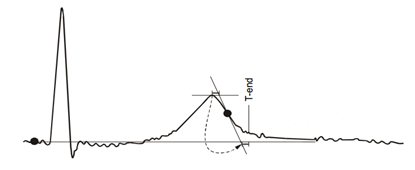
\includegraphics[scale=1.0]{QT_DISP/img/01}
\label{fig:Metoda 1}
\caption{Metoda stycznych}
\end{figure}

sposób drugi:
\begin{itemize}
  \item Odnalezienie punktu o maksymalnej prędkości na zstępującym ramieniu załamka T
  \item Wyznaczenie najlepiej dopasowanej paraboli do punktów chronologicznie późniejszych, ale poprzedzających globalnie wyznaczony koniec załamka T
  \item Wyznaczenie wierzchołka takiej paraboli jest tożsame ze znalezieniem końca załamka T.
\end{itemize}

Metoda ta prezentuje się następująco:
\begin{figure}[H]
\centering
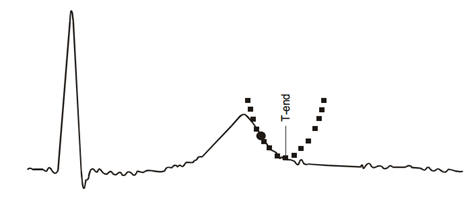
\includegraphics[scale=1.0]{QT_DISP/img/02}
\label{fig:Metoda 2}
\caption{Metoda parabol}
\end{figure}

\subsection{Rezultaty i wnioski}

W poniższej tabeli zaprezentowane są wyniki kilku obliczeń szerokości zespołów QT. 
\begin{figure}[H]
\centering
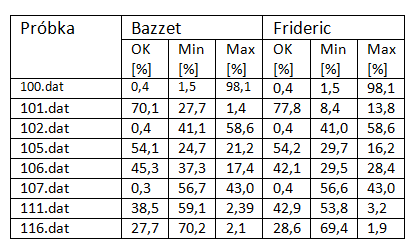
\includegraphics[scale=1.0]{QT_DISP/img/031}
\label{fig:Tabela1}
\caption{Tabela zawierająca opisy kilku przeprowadzonych eksperymentów : część 1}
\end{figure}

\begin{figure}[H]
\centering
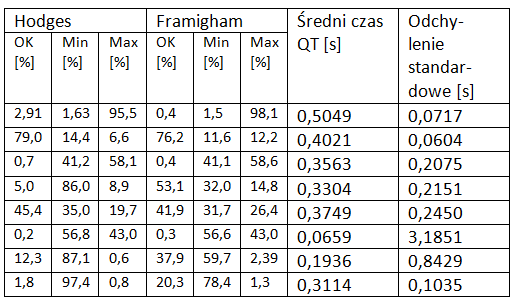
\includegraphics[scale=1.0]{QT_DISP/img/032}
\label{fig:Tabela2}
\caption{Tabela zawierająca opisy kilku przeprowadzonych eksperymentów : część 2}
\end{figure}

Gdzie: 

\begin{itemize}
  \item OK – prawidłowa długość załamka według danej ewaluacji [%]
  \item MAX – zbyt wielka długość załamka [%]
  \item MIN – zbyt mała długość załamka [%]
\end{itemize}

Poniżej też zaprezentowany jest na wykresie jeden zrzut ekranu z sygnału z oznaczonymi na nim końcami załamków T:
\begin{figure}[H]
\centering
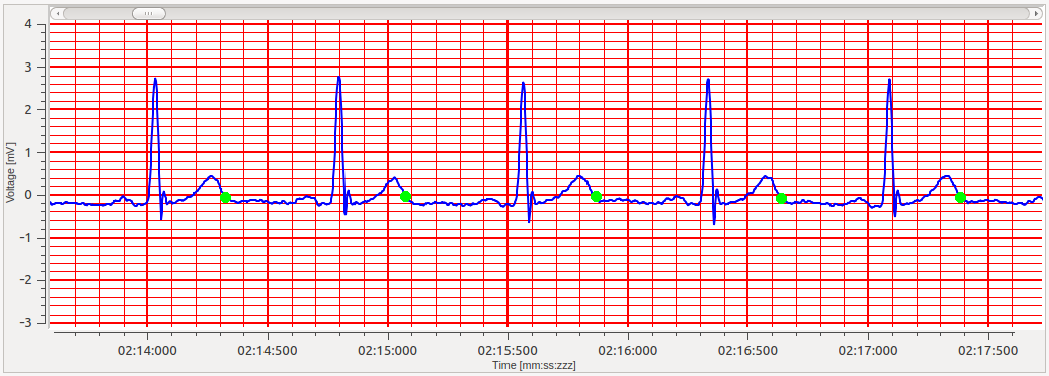
\includegraphics[scale=1.0]{QT_DISP/img/04}
\label{fig:Wykres1}
\caption{Przykładowe oznaczenie końców załamków T na wykresie EKG}
\end{figure}
